\chapter{Results}
\section{Results of the Baseline activity}
In the initial experiment, the baseline activity of the CA3 network was
observed from the \textit{original model} by
\textcite{sanjayImpairedDendriticInhibition2015}. The network was simulated for
5000 ms and showed synchronous activity throughout all three
populations (pyr, BC and OLM). Basket cells showed a higher firing rate
compared to the pyramidal cells and O-LM cells. The basket cells also swapped
between states of synchrony and asynchrony which was not observed in the other
two populations. The O-LM cells showed the lowest firing rate compared to the
pyramidal cells and basket cells. The baseline activity of the CA3 network is
shown in Figure~\ref{fig:baseline_activity}.

The average firing rates of the populations were 2.36 ± 0.024 Hz for pyramidal cells,
16.05 ± 0.15 Hz for basket cells, and 0.96 ± 0.027 Hz for O-LM interneurons,
similar to observed results from \textcite{neymotinKetamineDisruptsTheta2011} which used the same model on which the Sanjay model is based upon.

Just as reported in the original article, the network produces theta-modulated gamma oscillations
within the local field potential (LFP). These oscillations were influenced by signals from the Medial Septum (MS).
The gamma oscillations emerged from the inhibitory connections between basket cells that inhibit somas of pyramidal and O-LM cells,
as well as interactions among basket cells themselves. Conversely, theta oscillations were the result of interactions between
pyramidal cells and O-LM cells that inhibit dendrites. The network achieved a consistent theta frequency of 6.7 Hz due to periodic inputs
from the MS to both O-LM and basket cells every 150 ms. The frequency of the gamma component within the LFP was approximately 33 Hz.
Despite receiving similar MS inputs as O-LM cells, the impact on basket cells was significantly reduced because of their mutual interactions
and the enhanced influence from pyramidal cells.

\begin{figure}[htbp]
    \centering
    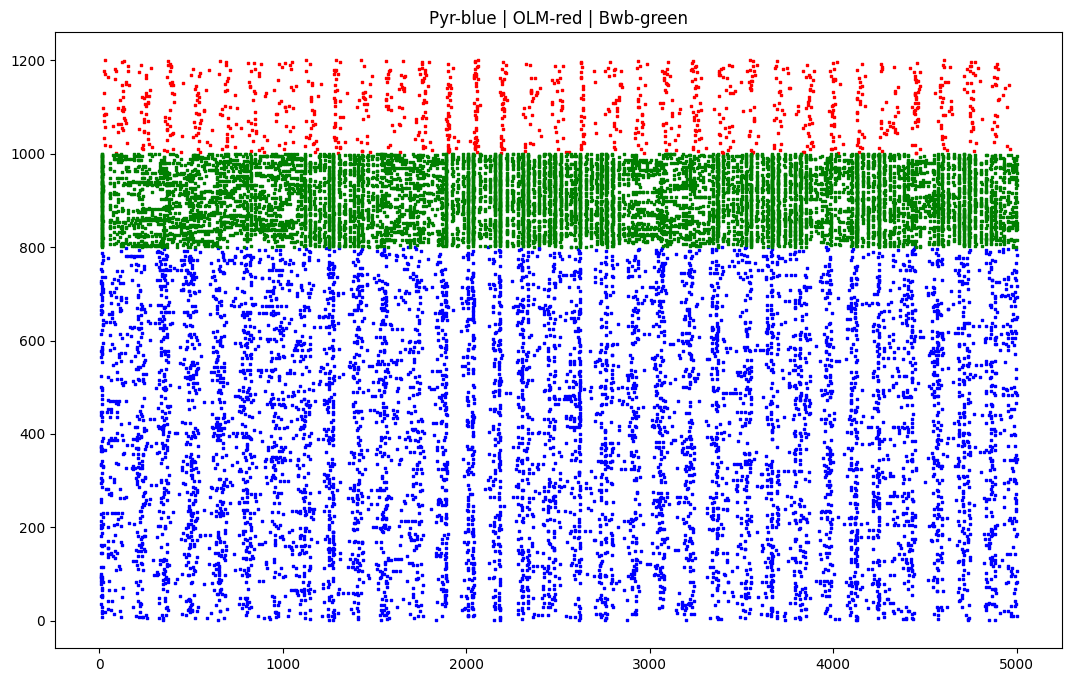
\includegraphics[width=1.0\textwidth]{Network_spike_activity_OLM_baseline.png}
    \caption[Baseline activity of the CA3 network]{Baseline activity of the CA3 network.
        The above figure shows the baseline activity of the CA3 network. The network was simulated for 5000 ms.
        The spike activity in time of the Pyr cells, BC cells, and OLM cells are shown based on the Neuron ID\@.
        ID 0--799 = Pyramidal (blue), 800--999 = BC (green), 1000--1200 = OLM (red).
        The x-axis represents the time in ms and the y-axis represents the neuron ID\@.}\label{fig:baseline_activity}
\end{figure}
\pagebreak
\section{Results of the Model validation}
To test whether our implementation of the CA3 network was able to replicate
more elaborate results, results from Figure 6 of the original
\textcite{sanjayImpairedDendriticInhibition2015} article were replicated in
Figure~\ref{fig:validation_firing_rates},~\ref{fig:validation_frequencies} and
~\ref{fig:validation_power}.

Like in the original experiment, O-LM-pyramidal connectivity was decreased in decrements of 0.1 and reduced dendritic inhibition.
Simultaneously, external noise fed to pyramidal cells via AMPA and NMDA at the synaptic level was increased in increments of 0.1.
When O-LM-pyramidal connectivity was decreased to a range of 20--10 \%, desynchronization was observed among basket cells (Figure~\ref{fig:scatterplot_20_con_olm_pyr}).
Complete desynchronization was observed when the O-LM-pyramidal connectivity was reduced to 0 \% (Figure~\ref{fig:scatterplot_0_con_olm_pyr}).
Pyramidal to O-LM connectivity was was unchanged, thus these cells showed sustained synchronous activity.

\begin{figure}[htbp]
    \centering
    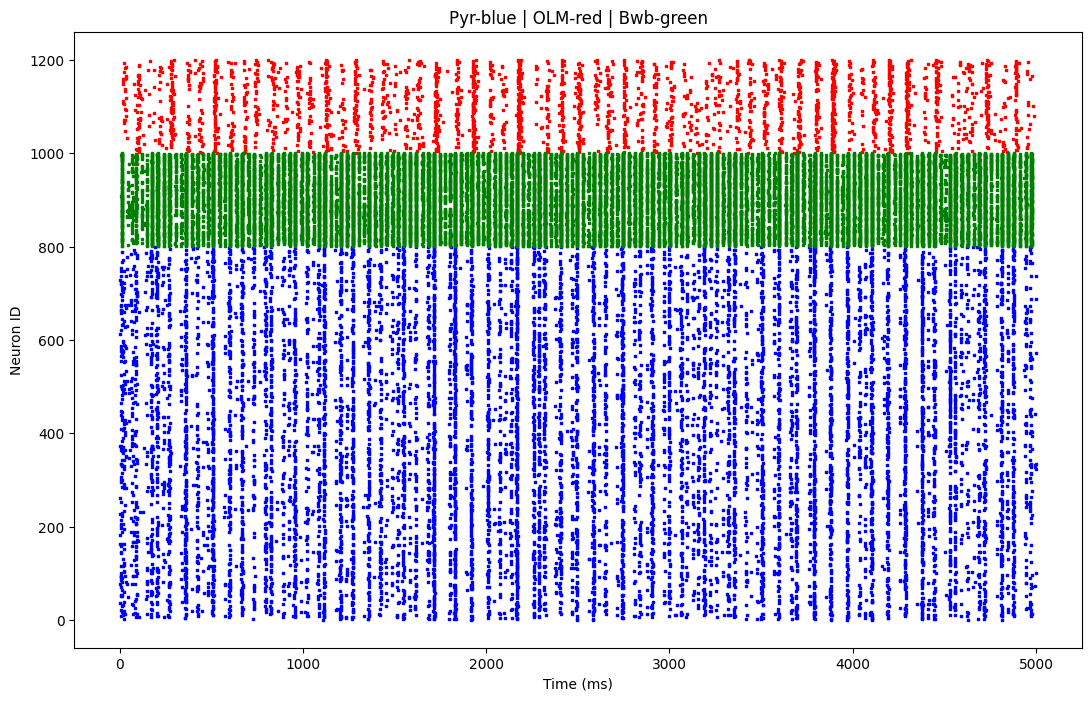
\includegraphics[width=1.0\textwidth]{Olm_pyr_20_con_scatter.png}
    \caption[20 \% OLM-Pyr connection scatter plot]{Scatter plot of the network activity at 20 \% OLM-Pyr connection
        The above figure shows the network activity at 20 \% OLM-Pyr connection with significant asynchrony amongst the basket cells.
        The network was simulated for 5000 ms.
        The scatter plot shows the spike activity of the Pyr cells (blue), BC cells (green), and OLM cells (red).
        The x-axis represents the time in ms and the y-axis represents the neuron ID\@.}\label{fig:scatterplot_20_con_olm_pyr}
\end{figure}

\begin{figure}[htbp]
    \centering
    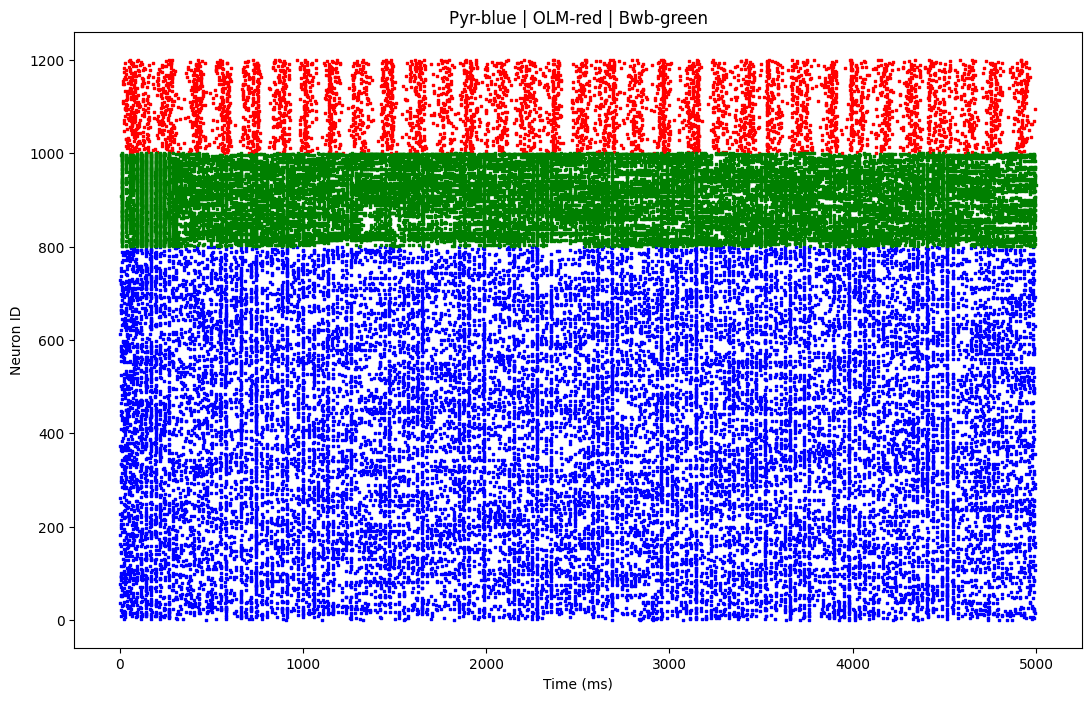
\includegraphics[width=1.0\textwidth]{Olm_pyr_no_connection_scatter.png}
    \caption[0 \% OLM-Pyr connection scatter plot]{Scatter plot of the network activity at 0 \% OLM-Pyr connection
        The above figure shows the network activity at 0 \% OLM-Pyr connection with complete asynchrony amongst the basket cells.
        The network was simulated for 5000 ms.
        The scatter plot shows the spike activity of the Pyr cells (blue), BC cells (green), and OLM cells (red).
        The x-axis represents the time in ms and the y-axis represents the neuron ID\@.}\label{fig:scatterplot_0_con_olm_pyr}
\end{figure}

The results show that the model was able to
replicate the results of the original article with slightly lower firing rates,
theta-gamma frequencies and power, which can be seen in
table~\ref{tab:validation_results}. The original article results are visible in
the methods section in table~\ref{tab:original_validation_results} for comparison.

For the firing rates in Figure~\ref{fig:validation_firing_rates},
there was a notable increase in the firing rates of all neuron types as dendritic inhibition was
decreased while external noise was simultaneously increased.
The individual cell firing frequencies showed a near linear increase throughout in both pyramidal and O-LM cells,
being most pronounced in the basket cell population.
The basket cell population also showed the most variance in the standard deviation at the most extreme
condition from the baseline (0.0x OLM-Pyr weight and 2.0x external weight).

The dominant frequencies in the network activity, as shown in Figure~\ref{fig:validation_frequencies},
showed that the theta frequency remained constant, while the gamma frequency only increased as dendritic inhibition was severely decreased and external noise increased.
The theta frequency remained constant at 6.2 Hz, slightly lower than the original model's 6.7 Hz, due to the strong pacing from the MS at this frequency.

The power of the theta and gamma oscillations in the network, as shown in Figure~\ref{fig:validation_power},
showed that the power of theta oscillations decreased, while the gamma power increased as dendritic inhibition was reduced.
This shift in power distribution reflects changes in the balance of network excitability and inhibition, potentially leading to epileptic activity.
The theta power reduced to 5.35 mV\textsuperscript{2} Hz\textsuperscript{-1} to 0 mV\textsuperscript{2} Hz\textsuperscript{-1}.
The gamma power increased significantly from at 20 to 10 \% O-LM-pyramidal connection. The gamma power increased from 0.93 mV\textsuperscript{2} Hz\textsuperscript{-1}
at baseline to 5.82 mV\textsuperscript{2} Hz\textsuperscript{-1} before dropping down to 1.87 mV\textsuperscript{2} Hz\textsuperscript{-1} in the last condition.
The gamma power was mostly due to basket cell activity, which were much more tightly synchronized than the other cell types.

The trends in the original figures were similar in Figure~\ref{fig:validation_original_results} to the ones of this section.
Therefore, it was assumed that the model was correctly implemented and the results were valid.

\begin{figure}[htbp]
    \centering
    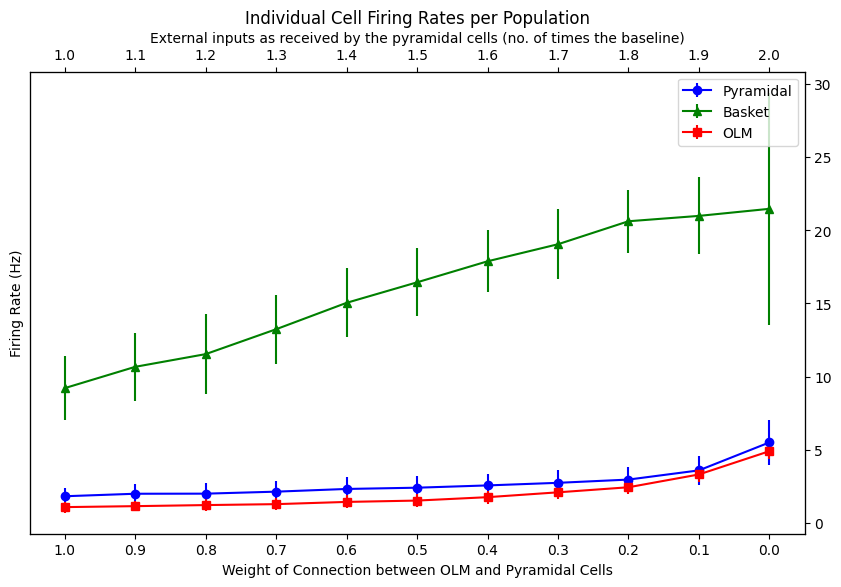
\includegraphics[width=1.0\textwidth]{Sanjay_validation_firing_rates.png}
    \caption[Validation: Firing rates per population]{Validation of the firing rates.
        The above figure shows the firing rates of the Pyr cells, BC cells, and O-LM cells when dendritic inhibition is decreased and external noise is increased.
        The firing rates were calculated from the spike activity of the cells in each population for the duration of the simulation (5000 ms).
        The double x-axis represents both decrement in the weight of dendritic inhibition on pyramidal cells by OLM interneurons,
        while simultaneously increasing external noise stimulation to pyramidal cells.
        External noise levels rise and inhibition decreases by increments of 0.1, each representing a 10\% change relative to the baseline.
        The y-axis represents the firing rate in Hz.
        The firing rates are per cell type: Pyr (blue), Basket (green) and OLM (red).
        The error bars represent the standard deviation of the firing rates.}\label{fig:validation_firing_rates}
\end{figure}

\begin{figure}[htbp]
    \centering
    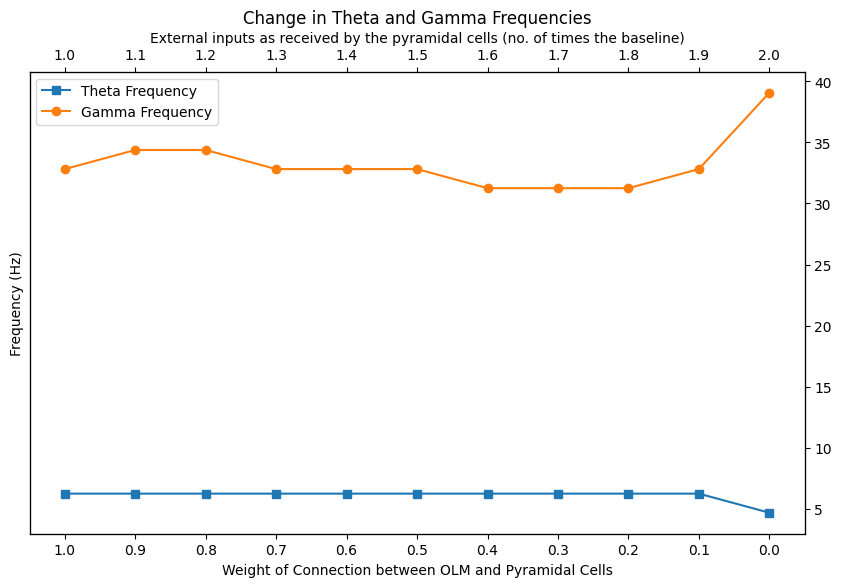
\includegraphics[width=1.0\textwidth]{Sanjay_validation_frequencies.png}
    \caption[Validation: Dominant frequencies]{Validation of dominant frequencies.
        The above figure shows the dominant theta-gamma frequencies in the network activity when dendritic inhibition is decreased and external noise is increased.
        The double x-axis represents both decrement in the weight of dendritic inhibition on pyramidal cells by O-LM interneurons,
        while simultaneously increasing external noise stimulation to pyramidal cells.
        External noise levels rise and inhibition decreases by increments of 0.1, each representing a 10\% change relative to the baseline.
        The y-axis represents the dominant frequency in Hz for both theta (3--12 Hz, blue) and gamma (30--80 Hz, orange) oscillatory bands.}\label{fig:validation_frequencies}
\end{figure}

\begin{figure}[htbp]
    \centering
    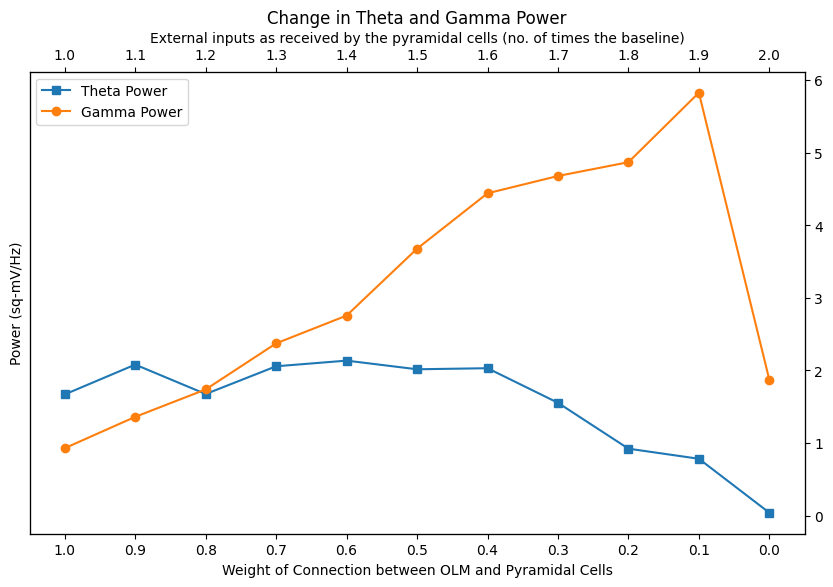
\includegraphics[width=1.0\textwidth]{Sanjay_validation_power.png}
    \caption[Validation: Theta-Gamma power]{Validation of Theta-Gamma power.
        The above figure shows the power of the theta and gamma oscillations in the network when dendritic inhibition is decreased and external noise is increased.
        The double x-axis represents both decrement in the weight of dendritic inhibition on pyramidal cells by O-LM interneurons,
        while simultaneously increasing external noise stimulation to pyramidal cells.
        External noise levels rise and inhibition decreases by increments of 0.1, each representing a 10\% change relative to the baseline.
        The y-axis represents the theta and gamma power (blue and orange, respectively).}\label{fig:validation_power}
\end{figure}

\begin{table}[htbp]
    \centering
    \caption[Summary of Model validation: Network simulation Parameters and Results]{Overview of Model Validation Network Simulation Settings and Outcomes.
        Variations in the firing rates of cell populations, alongside theta and gamma oscillations within the local field potential, as well as the alterations in their intensity upon the decrease of dendritic inhibition and the concurrent enhancement of external stimuli to the pyramidal neurons.}\label{tab:validation_results}
    \begin{adjustbox}{width=\textwidth}
        \begin{tabular}{ccccccccc}
            \hline
            OLM-Pyr Wt & External Wt & \CellWithForcedBreak{Pyr (Hz)                                                     \\ + Std} & \CellWithForcedBreak{BWB (Hz) \\ + Std} & \CellWithForcedBreak{OLM (Hz) \\ + Std} & \CellWithForcedBreak{Theta \\ Freq (Hz)} & \CellWithForcedBreak{Theta power \\ (mV\textsuperscript{2} Hz\textsuperscript{-1})} & \CellWithForcedBreak{Gamma \\ Freq (Hz)} & \CellWithForcedBreak{Gamma power \\ (mV\textsuperscript{2} Hz\textsuperscript{-1})} \\
            \hline
            1.0X       & 1.0X        & 1.83±0.58                     & 9.21±2.20  & 1.08±0.38 & 6.2 & 1.67 & 32.8 & 0.93 \\
            0.9X       & 1.1X        & 2.00±0.64                     & 10.67±2.31 & 1.15±0.36 & 6.2 & 2.08 & 34.4 & 1.36 \\
            0.8X       & 1.2X        & 2.00±0.71                     & 11.54±2.72 & 1.22±0.39 & 6.2 & 1.67 & 34.4 & 1.74 \\
            0.7X       & 1.3X        & 2.14±0.74                     & 13.24±2.36 & 1.29±0.42 & 6.2 & 2.06 & 32.8 & 2.37 \\
            0.6X       & 1.4X        & 2.33±0.79                     & 15.04±2.35 & 1.44±0.45 & 6.2 & 2.13 & 32.8 & 2.76 \\
            0.5X       & 1.5X        & 2.41±0.80                     & 16.44±2.31 & 1.53±0.45 & 6.2 & 2.02 & 32.8 & 3.68 \\
            0.4X       & 1.6X        & 2.57±0.79                     & 17.88±2.12 & 1.76±0.45 & 6.2 & 2.03 & 31.2 & 4.44 \\
            0.3X       & 1.7X        & 2.74±0.86                     & 19.04±2.38 & 2.10±0.49 & 6.2 & 1.55 & 31.2 & 4.68 \\
            0.2X       & 1.8X        & 2.97±0.88                     & 20.61±2.14 & 2.44±0.48 & 6.2 & 0.92 & 31.2 & 4.87 \\
            0.1X       & 1.9X        & 3.59±0.99                     & 20.98±2.62 & 3.31±0.50 & 6.2 & 0.78 & 32.8 & 5.82 \\
            0.0X       & 2.0X        & 5.50±1.52                     & 21.46±7.93 & 4.90±0.52 & 4.7 & 0.04 & 39.1 & 1.87 \\
            \hline
        \end{tabular}
    \end{adjustbox}
\end{table}
\pagebreak
\section{Results of the Sodium-Potassium variants}
In this experiment, the sodium and potassium conductance of the pyramidal, basket, and O-LM cells were modified in increments of 0.1.
This was done in a range of 0.5 to 1.5 times the baseline conductance.
Similarly to the previous experiment, the network was simulated for 5000 ms and the firing rates, dominant frequencies, and power of the theta and gamma oscillations were calculated in Figures~\ref{fig:sodium_potassium_firing_rates},~\ref{fig:sodium_potassium_frequencies} and~\ref{fig:sodium_potassium_power}, respectively.

\begin{figure}[htbp]
    \centering
    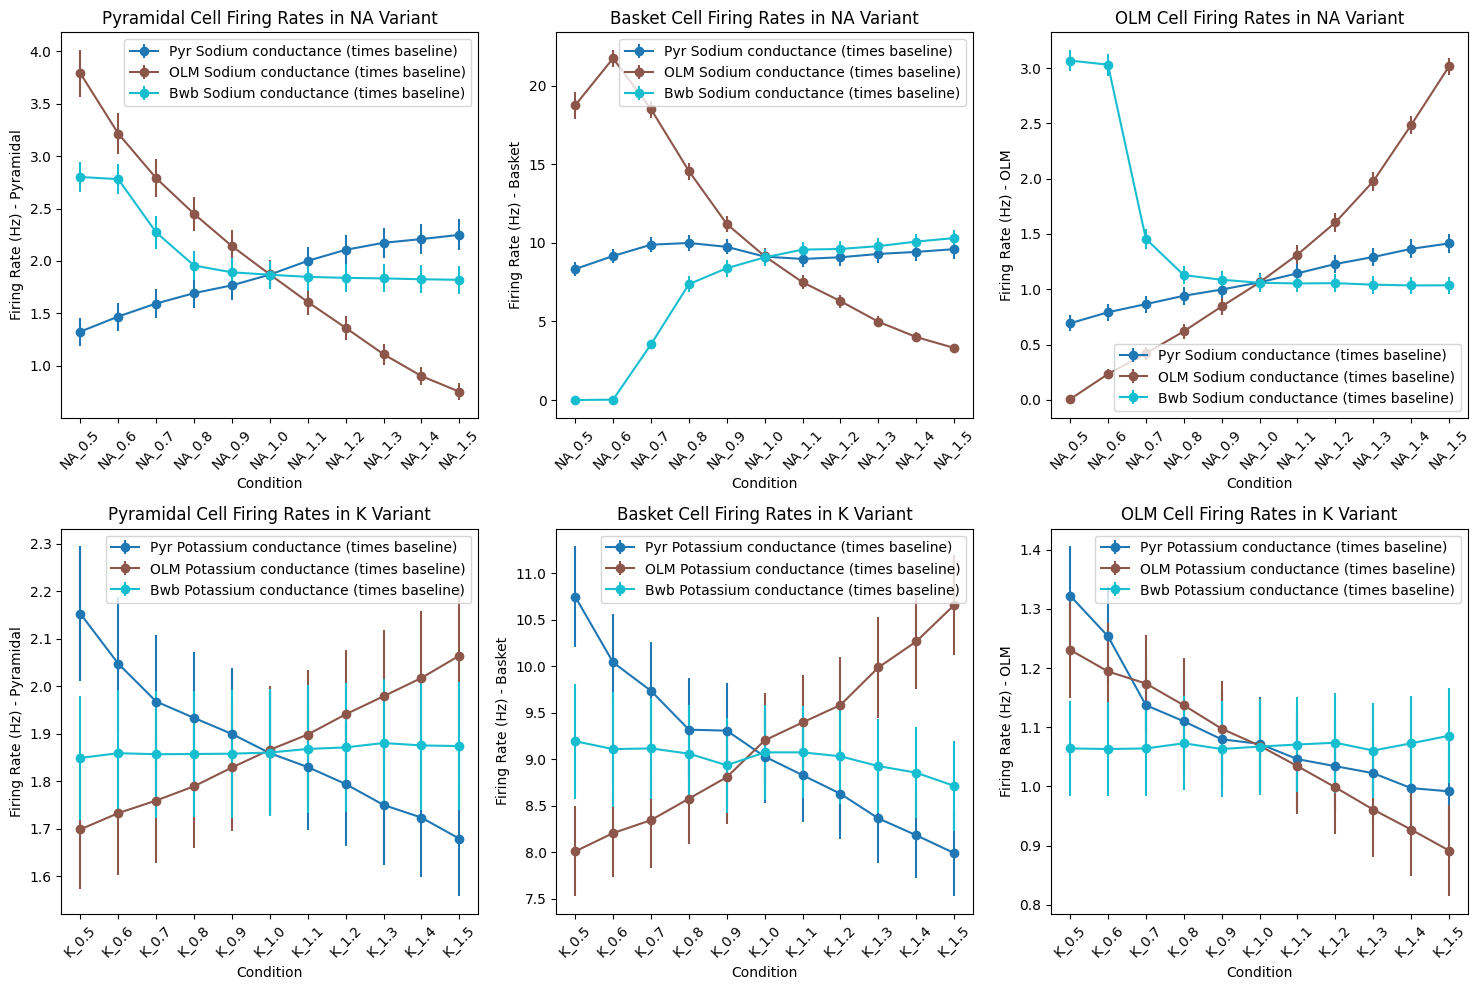
\includegraphics[width=1.0\textwidth]{Cell_firing_rates_per_pop_per_variant.png}
    \caption[Sodium-Potassium variants: Firing rates per population]{Sodium-Potassium variants: Firing rates per population.
        The above figure shows the firing rates of the Pyr cells, BC cells, and O-LM cells for each modified cell type.
        Each of the three cell types either had modified sodium or potassium conductance.
        The firing rates were calculated from the spike activity of the cells in each population for the duration of the simulation (5000 ms).
        The x-axis represents the percentage amount of changed sodium or potassium conductance, times the baseline.
        The y-axis represents the firing rate in Hz.
        The firing rates are per cell type: Pyr (blue), Basket (cyan) and OLM (red).
        The error bars represent the standard error of the mean (SEM) of the firing rates per population.}\label{fig:sodium_potassium_firing_rates}
\end{figure}

\subsection{Firing rates: Pyramidal cells}
In Figure~\ref{fig:sodium_potassium_firing_rates}, the firing rates of pyramidal cells showed the largest change when the sodium conductance (\(g_{\text{Na}}\)) of O-LM cells was modified.
When the sodium conductance of O-LM cells (dendrite-inhibiting) was decreased, the firing rate of pyramidal cells increased, and vice versa.
Sodium conductance of basket cells (soma-inhibiting) was also modified. Interestingly, the firing rate of pyramidal cells was unaffected when \(g_{\text{Na}}\) was increased.
However, when \(g_{\text{Na}}\) was decreased by more than 30 \% the firing rate of pyramidal cells increased sharply.
Lastly, increasing the \(g_{\text{Na}}\) in the pyramidal cells themselves led only to a marginal in- and decrease in firing rates.

Changing the potassium conductance (\(g_{\text{K}}\)) had more profound effects on pyramidal firing rates.
When the potassium conductance of O-LM cells was increased, the firing rate of pyramidal cells decreased, and vice versa.
Changing \(g_{\text{K}}\) of basket cells had almost no effect on the firing rate of pyramidal cells.
However, when the potassium conductance of pyramidal cells was modified, the effect of potassium on the pyramidal firing rates were almost the exact opposite of modified the O-LM cells.

\subsection{Firing rates: Basket cells}
Compared to pyramidal cell firing rates, the basket cell population has some significantly different trends in firing rates.
When the \(g_{\text{Na}}\) of O-LM cells was modified, the firing rate of basket cells decreased, and vice versa.
Interestingly, at -40 \% \(g_{\text{Na}}\) of O-LM the firing rate peaks and then decreases sharply, instead of a linear decrease.
Changing the \(g_{\text{Na}}\) of pyramidal cells had barely any effect on the firing rate of basket cells.
Whereas changing the \(g_{\text{Na}}\) of basket cells themselves, led to a sharp decrease in firing rate at -30 \% \(g_{\text{Na}}\) and a complete loss of firing at a -40 \%  \(g_{\text{Na}}\).
Generally, the firing rates were much higher and the effects on the firing rates were more pronounced compared to the pyramidal cells and O-LM cells (with the largest SEM).

Changing the \(g_{\text{K}}\) of basket cells had a similar effect to that of pyramidal population, albeit with larger in- and decreases in Hz.
Just like the pyramidal firing rates, the basket firing rate increases when O-LM \(g_{\text{K}}\) is increased and vice versa.
The firing rate of basket cells was unaffected when the \(g_{\text{K}}\) of basket cells was modified.
Whereas increasing the \(g_{\text{K}}\) of pyramidal cells led to a decrease of basket cell firing rate and vice versa.

\subsection{Firing rates: O-LM cells}
The O-LM population showed the most unique variations in firing rates.
When the \(g_{\text{Na}}\) of O-LM cells was modified, the firing rate of O-LM cells increased, and vice versa.
However, when the \(g_{\text{Na}}\) of basket cells was decreased below -30 \%, the firing rate of O-LM cells increased sharply to more than double the Hz.
Pyramidal \(g_{\text{Na}}\) had a a weak and linear effect on the O-LM firing rates, where increased \(g_{\text{Na}}\) led to increased firing rates and decreased \(g_{\text{Na}}\) led to decreased firing rates.

Changing the \(g_{\text{K}}\) of O-LM cells had an inverted effect on firing rates compared to \(g_{\text{Na}}\).
Modifications to basket cell \(g_{\text{K}}\), again, had little to no effect on the firing rate of O-LM cells.
However, when the \(g_{\text{K}}\) of pyramidal cells was modified, the effect on the O-LM firing rates was almost the same as the O-LM \(g_{\text{K}}\) modifications.
\pagebreak

\subsection{Dominant frequencies}
In this experiment the dominant theta and gamma frequencies were identified from the local field potential (LFP) for the duration of the simulation (5000 ms) by performing a power spectrum density analysis.
The dominant frequencies were calculated for each modified cell type and are shown in Figure~\ref{fig:sodium_potassium_frequencies}.
The figure is split in both sodium and potassium conductance modifications for each cell type (pyramidal = blue, OLM = red, basket = cyan).

\begin{figure}[htbp]
    \centering
    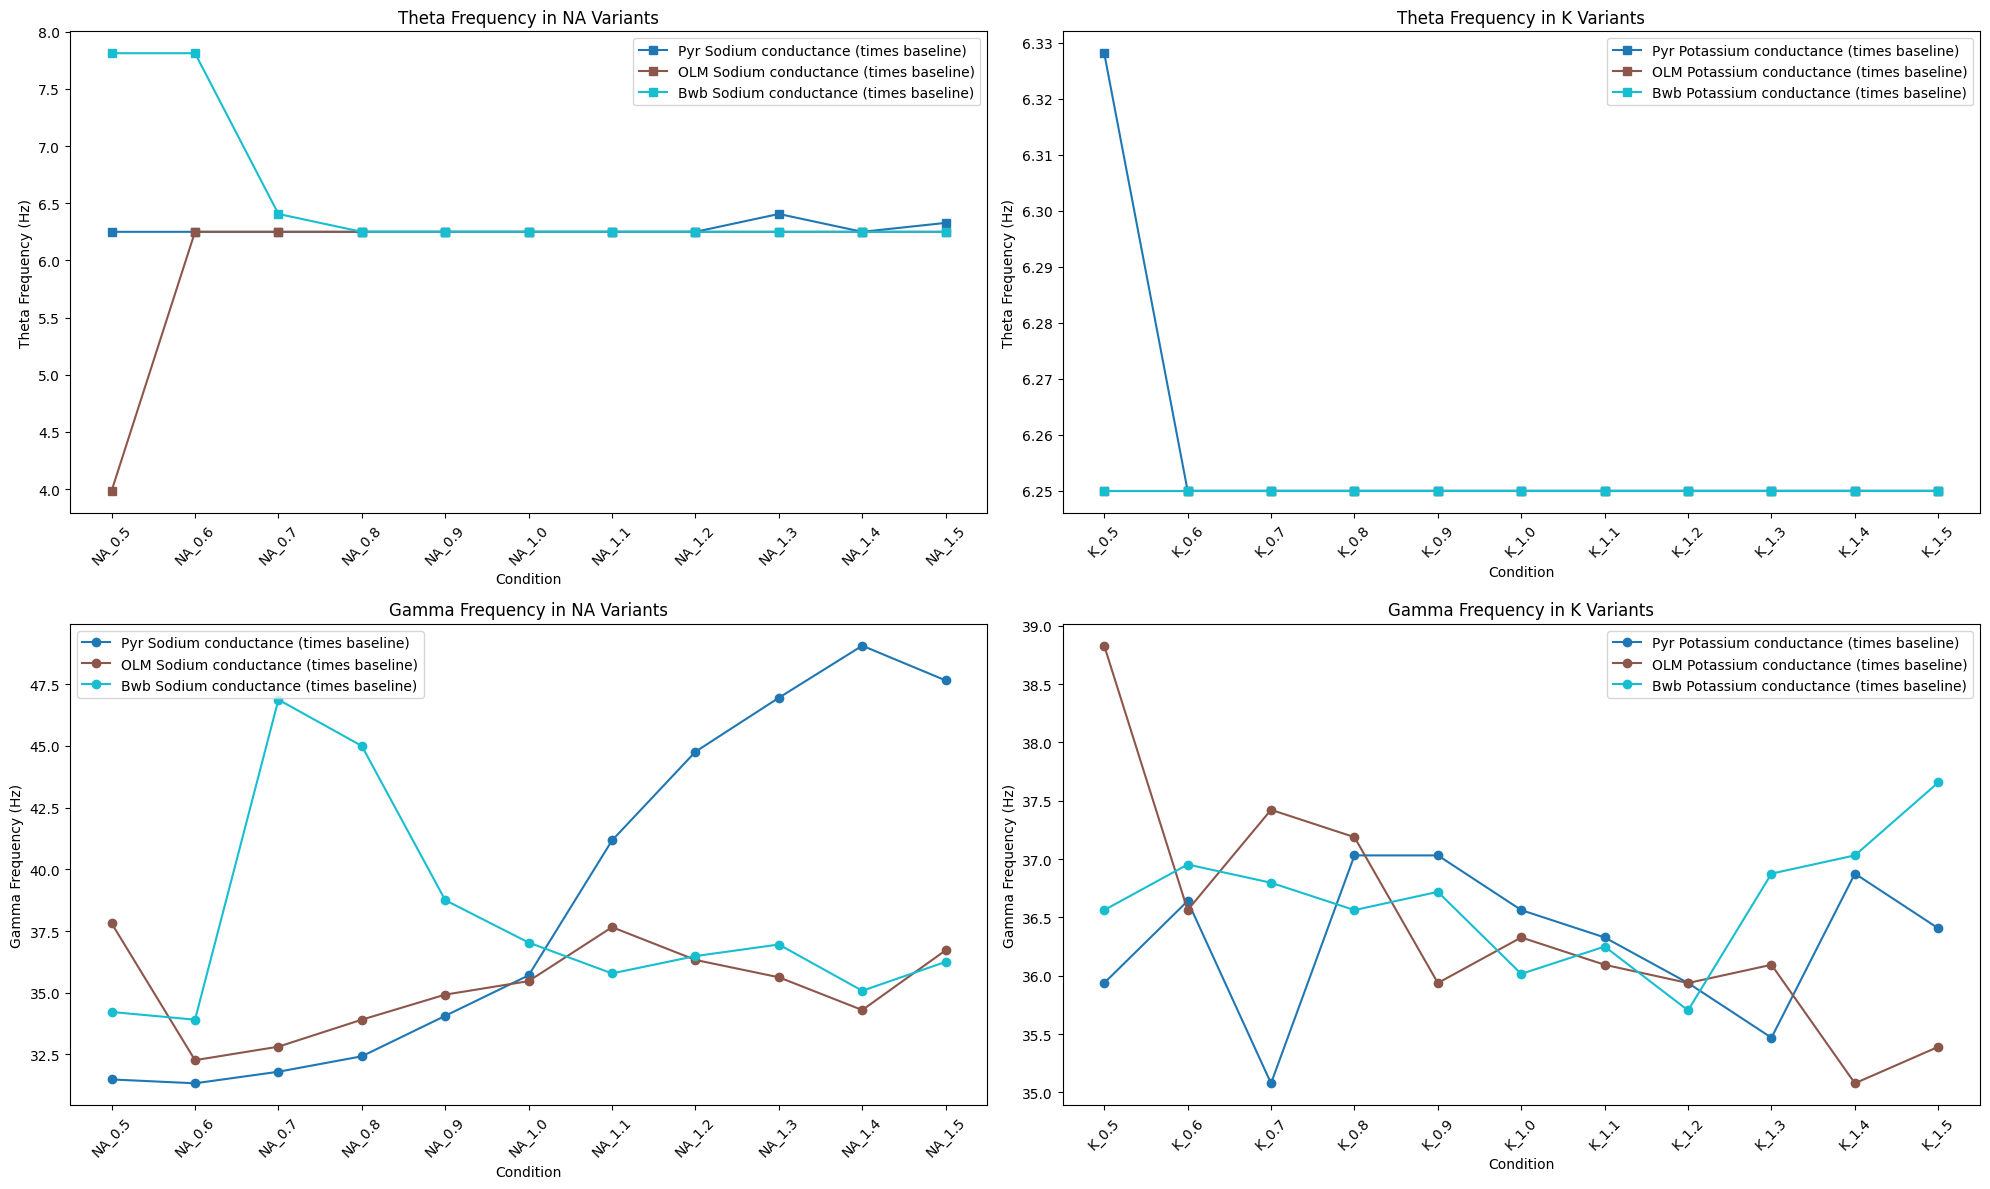
\includegraphics[width=1.0\textwidth]{Theta_gamma_freqs_variants.png}
    \caption[Sodium-Potassium variants: Dominant frequencies]{Sodium-Potassium variants: Dominant frequencies.
        The above figure shows the dominant theta-gamma frequencies in the network activity for each modified cell type.
        Each of the three cell types either had modified sodium or potassium conductance (pyr = blue, OLM = red, basket = cyan).
        The dominant frequencies were calculated from the local field potential (LFP) for the duration of the simulation (5000 ms).
        The x-axis represents the percentage amount of changed sodium or potassium conductance, times the baseline.
        The y-axis represents the dominant frequency in Hz for both theta (3--12 Hz) and gamma (30--80 Hz) oscillatory bands.}\label{fig:sodium_potassium_frequencies}
\end{figure}

\subsubsection{Theta frequency}
For both sodium and potassium conductance modifications, the theta frequency was largely unaffected as it is generated by the strong pacemaker influence of the medial septum at the 6.2 Hz frequency.
There were a couple of outliers in both conditions, in the -50 \% conditions of O-LM and basket \(g_{\text{Na}}\), is decreased and increased respectively (\ref{fig:sodium_potassium_frequencies}, top left = sodium theta, right = potassium theta).

\subsubsection{Gamma frequency}
Conversely, the gamma frequency was more affected by the sodium and potassium conductance modifications.
In the modified pyramidal condition the gamma frequency increased sharply from -50 \% to 50 \% \(g_{\text{Na}}\) from 30.4 hz to 48,8 Hz.
O-LM modifications in comparison, had a less significant effect on the gamma frequency, with a slight increase from the baseline at 10 \% increased \(g_{\text{Na}}\).
Basket cell modifications had the most significant effect on the gamma frequency, with a sharp increase of more than 10 Hz from -40 \% \(g_{\text{Na}}\) to -30\%.
It sharply decreases nearing baseline, at which increased \(g_{\text{Na}}\) of basket cells had very little effect on the gamma frequency (\ref{fig:sodium_potassium_frequencies}, bottom left).

The effects of potassium on gamma frequency seems to more random without a clear trend in in- or decrease of conductance for all cell types.
Each increment of 0.1 appeared to have a different effect on the gamma frequency, with some conditions showing a sharp increase or decrease in Hz.
The the power of the gamma frequency stayed mostly within the 35.5 to 37.5 Hz range (\ref{fig:sodium_potassium_frequencies}, bottom right).
\subsection{Theta-gamma power}
Another aspect of the sodium-potassium experiment was a power analysis of the theta and gamma oscillations in the network based on the power spectrum density.
The power of the theta and gamma oscillations were calculated from the local field potential (LFP) for the duration of the simulation (5000 ms) and are shown in Figure~\ref{fig:sodium_potassium_power}.
The figure is again split in both sodium and potassium conductance modifications for each cell type (pyramidal = blue, OLM = red, basket = cyan).

\begin{figure}[htbp]
    \centering
    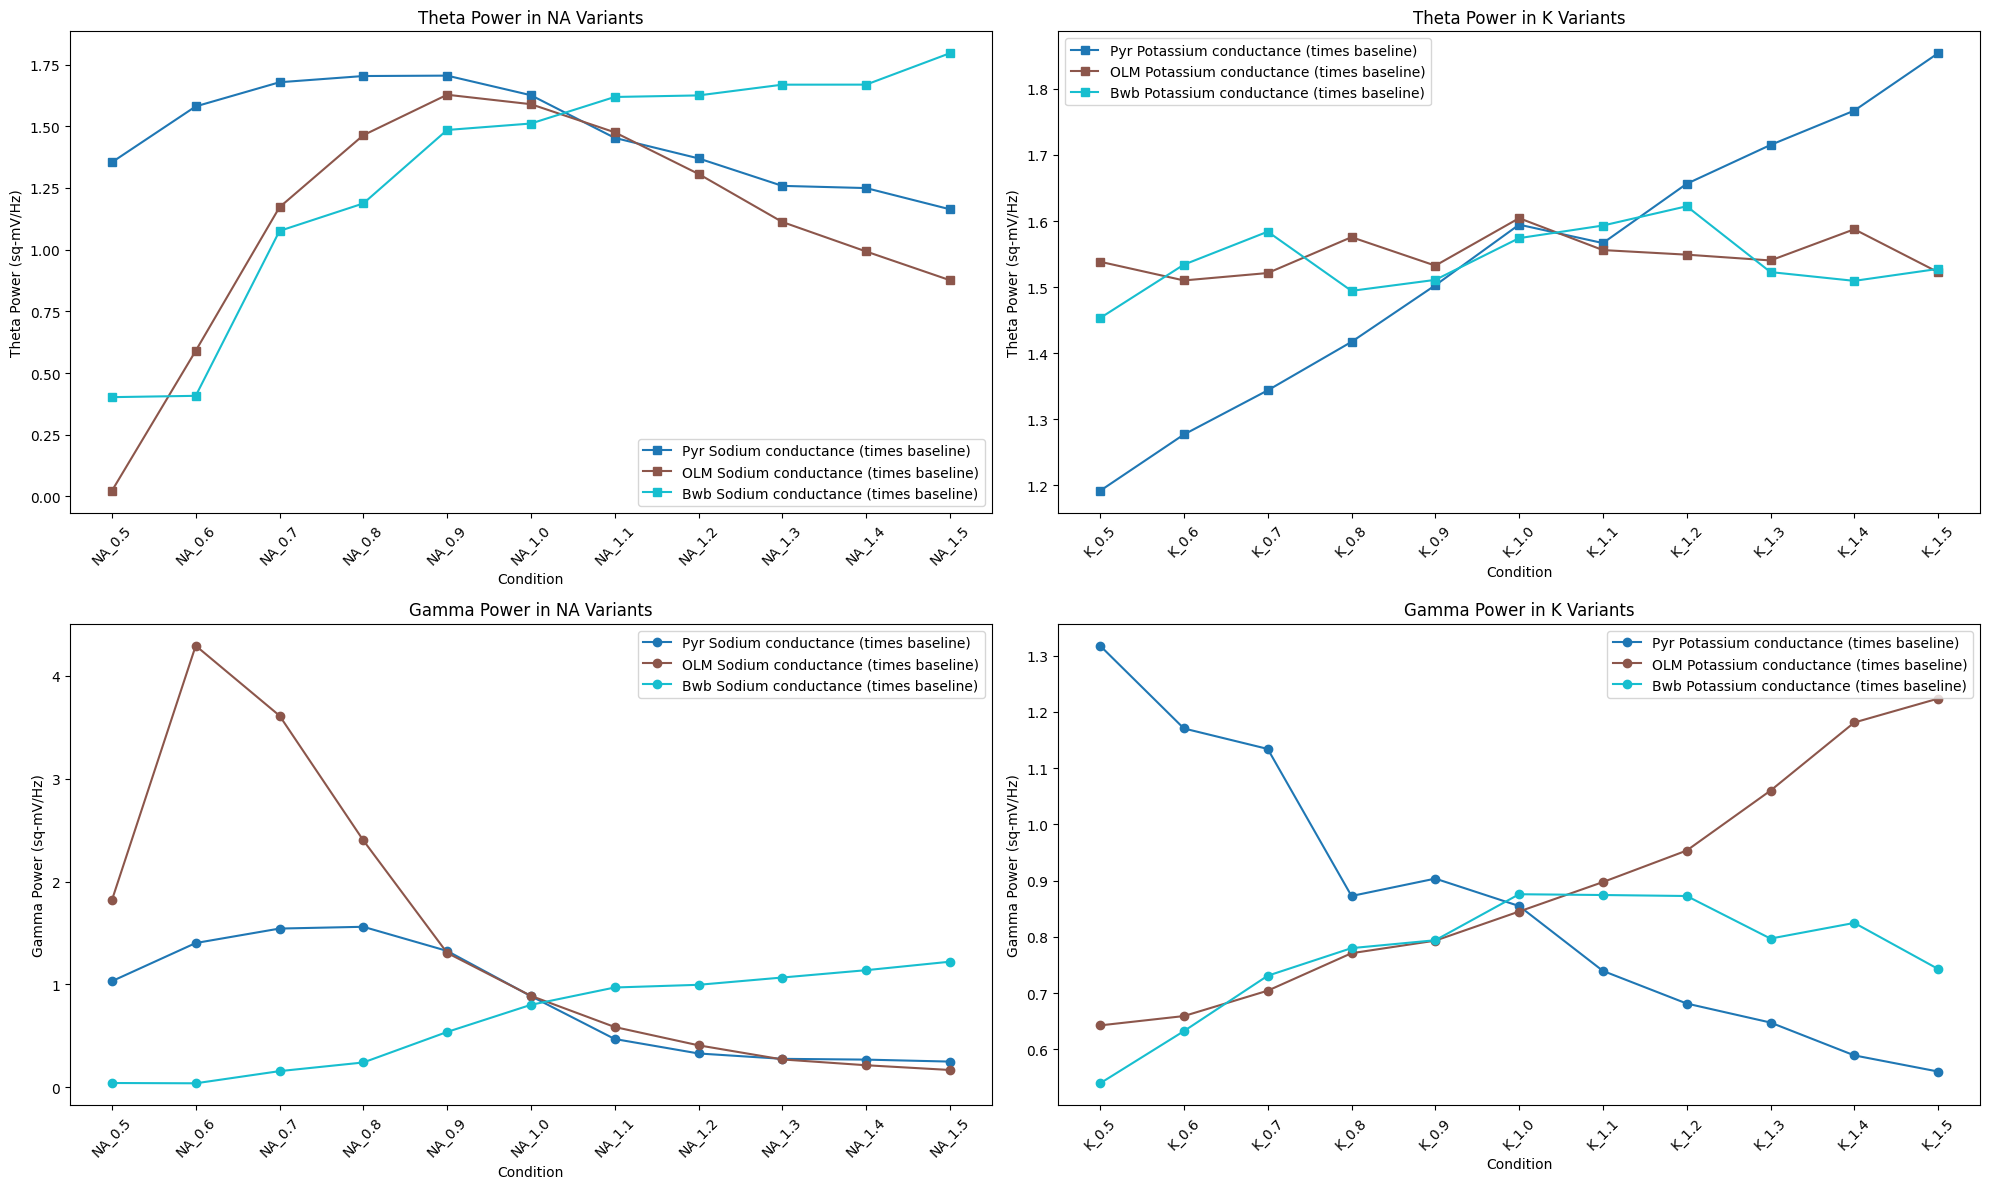
\includegraphics[width=1.0\textwidth]{Theta_gamma_power_variants.png}
    \caption[Sodium-Potassium variants: Theta-Gamma power]{Sodium-Potassium variants: Theta-Gamma power.
        The above figure shows the power of the theta and gamma oscillations in the network for each modified cell type.
        Each of the three cell types either had modified sodium or potassium conductance (pyr = blue, OLM = red, basket = cyan).
        The power of the theta and gamma oscillations were calculated from the local field potential (LFP) for the duration of the simulation (5000 ms).
        The x-axis represents the percentage amount of changed sodium or potassium conductance, times the baseline.
        The y-axis represents the theta and gamma power (in mV\textsuperscript{2} Hz\textsuperscript{-1}).}\label{fig:sodium_potassium_power}
\end{figure}

\subsubsection{Theta power}
Theta power showed an rising trend in all three cell types where O-LM and basket cells had the most significant increase in power in below-baseline conditions.
This change in power occurred predominantly in the -50 \% to -30 \% \(g_{\text{Na}}\) range.
After which, O-LM falls off together with the modified pyramidal condition and decreases slightly.
The basket cell condition shows the relative highest theta power above baseline conditions and remained slightly above baseline (\ref{fig:sodium_potassium_power}, top left).

In the modified potassium conductance conditions only the pyramidal modifications had an almost linear increase in theta power from -50 \% to +50 \% \(g_{\text{K}}\).
Modifications in the other cell types remained fairly constant in theta power (\ref{fig:sodium_potassium_power}, top right).

\subsubsection{Gamma power}
Unlike the frequency, the power of the gamma oscillations showed a large spike in power when the O-LM cells were modified from -50 \% to -40 \% \(g_{\text{Na}}\) of almost double the power.
The effect of which in the LFP power spectrum is visualized using a fast-Fourier transformation in Figure~\ref{fig:comparative_fft_olm_variant}.
From this figure, it is clear that some conditions cause significant shifts in gamma power at specific frequencies (30--40 Hz and 60--70 Hz).
The gamma power sharply drops back to a more constant level from baseline onwards.
The other cell types show a shift from 1 and 0 Hz to 0 and 1 Hz for Pyramidal and Basket cell modified conditions respectively (\ref{fig:sodium_potassium_power}, bottom left).

Increased \(g_{\text{K}}\) of O-LM cells from -50 \% onwards resulted in a constant rise in gamma power in the network, whereas modifications in pyramidal populations resulted in a steady decrease in gamma power.
Basket cell modifications had a more random effect on gamma power, with some more extreme conditions reduced gamma power compared to baseline (\ref{fig:sodium_potassium_power}, bottom right).

\begin{figure}[htbp]
    \centering
    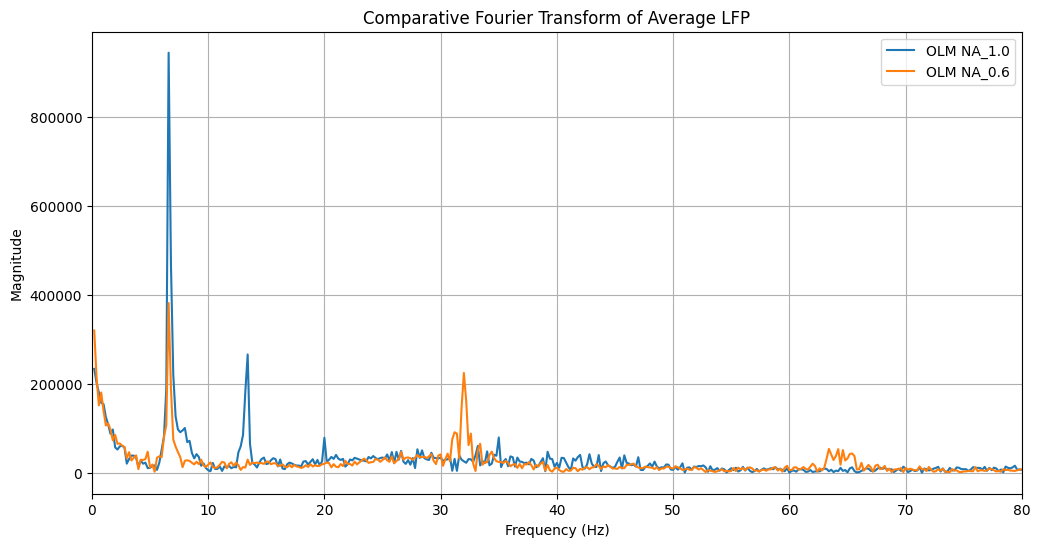
\includegraphics[width=1.0\textwidth]{Comparative_FFT_LFP_OLM_variant.png}
    \caption[Comparative FFT of LFP\@: O-LM variants]{Comparative FFT of the LFP for OLM variants.
        The magnitude of the LFP is in arbitrary units.
        The signal is plotted for the frequency range that includes both theta and gamma in a range of 0 to 80 Hz.
        Blue is the baseline LFP, whereas orange represents a -40 \% sodium conductance variant of O-LM cells.}\label{fig:comparative_fft_olm_variant}
\end{figure}

\pagebreak

\section{Results of the External Noise variants}
As a follow-up to the sodium-potassium experiment, the network's sensitivity to a range of external noise conditions was tested for different combinations of modified pyramidal sodium/potassium conductance.
The occurrence of depolarization block events in basket cells were quantified, including the average delay of these events in trials where they occurred.
The external noise fed to the pyramidal cells was modified in increments of 0.05, ranging from 0.65 to 0.95 times the baseline noise level.\\

\noindent More noise conditions are available for review in appendix~\ref{ch:appendix_c}.

\subsection{Occurrence of depolarization block events across noise conditions}
To test the susceptibility of the network to depolarization block (DPB) events, the percentage of trials where DPB events occurred was calculated in Figure~\ref{fig:dpb_percentage_matrices}.
The color intensity of the matrices indicate how often the network entered an epileptic state per noise condition for different combinations of pyramidal cell modifications of sodium and potassium.
At baseline sodium-potassium conductance and 20 times noise the network response is visible with a clear depolarization block in basket cells in Figure~\ref{fig:scatterplot_1_con_olm_pyr_ext_noise_20x}.

In matrix a in Figure~\ref{fig:dpb_percentage_matrices}, there were barely any DPB events in the 15 trials per condition. Most of the DPB events occurred near baseline \(g_{\text{Na}}\) and \(g_{\text{K}}\) conditions and with elevated \(g_{\text{K}}\) only.

In matrix b, the number of DPB events increased significantly, with the most events occurring at elevated pyramidal sodium conductance conditions.

Matrix c showed a similar trend to matrix b, with more DPB events occurring also at more severely elevated pyramidal potassium conductance conditions.

Matrix d showed the most DPB events, with the most events occurring at elevated pyramidal sodium conductance conditions with the exception of severely reduced sodium and potassium conductance combinations (bottom left).
The selected noise levels are a percentage of the fixed 20x times baseline external noise level (0.65, 0.75, 0.85, 0.95).

\begin{figure}[htbp]
    \centering
    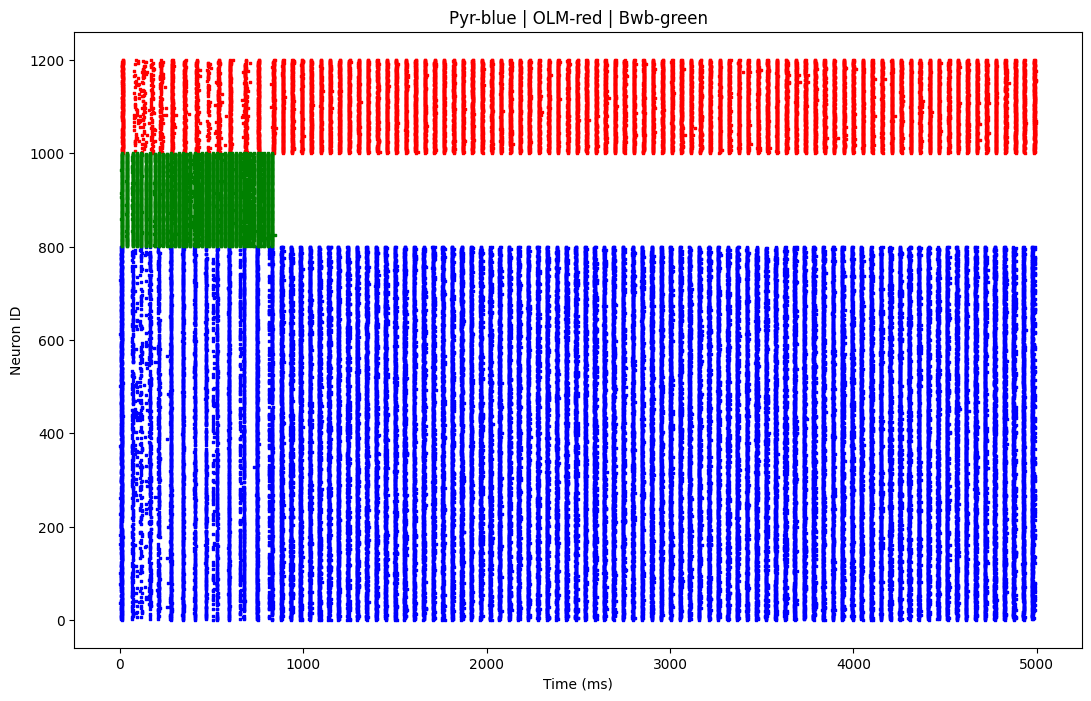
\includegraphics[width=1.0\textwidth]{ictal_tonic_baseline_noise_20x_0.10_OLM_pyr.png}
    \caption[10 \% O-LM-Pyr connection with increased external noise scatter plot]{Scatter plot of the network activity at 10 \% O-LM-Pyr connection with increased external noise (20x times baseline).
        The above figure shows the network activity at 10 \% O-LM-Pyr connection with a depolarization block in the basket cell population.
        There is a clear ictal-tonic pattern in the population activity, along with very high synchronous spiking between O-LM and Pyr cells.
        The network was simulated for 5000 ms.
        The scatter plot shows the spike activity of the Pyr cells (blue), BC cells (green), and O-LM cells (red).
        The x-axis represents the time in ms and the y-axis represents the neuron ID\@.}\label{fig:scatterplot_1_con_olm_pyr_ext_noise_20x}
\end{figure}
\pagebreak

\begin{figure}[htbp]
    \centering
    % Row 1
    \begin{subfigure}{0.48\textwidth}
        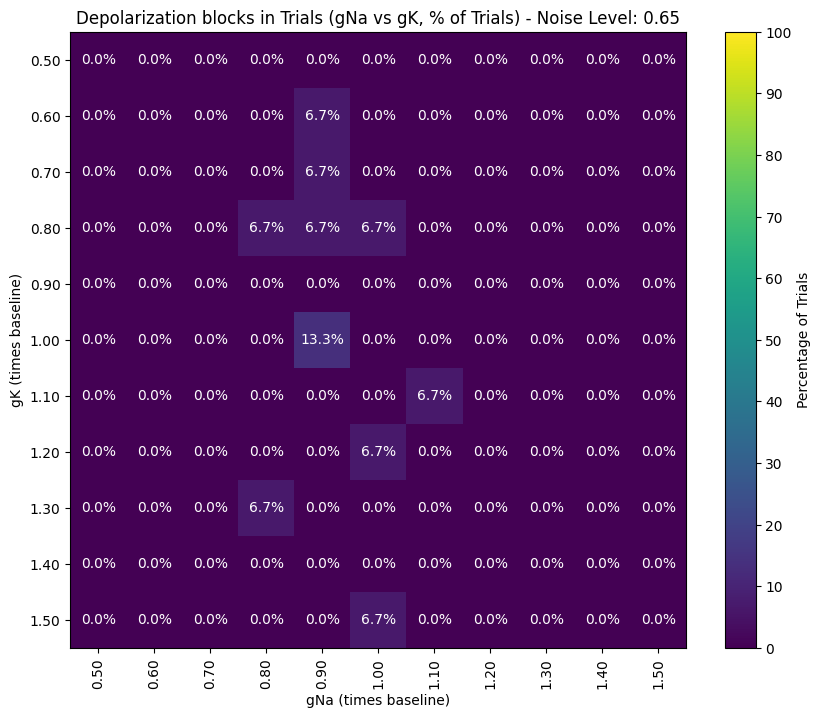
\includegraphics[width=\linewidth]{DPB_percentage_matrices/DPB_percentage_noise_0.65.png}
        \caption{} % Optional caption
    \end{subfigure}\hfill
    \begin{subfigure}{0.48\textwidth}
        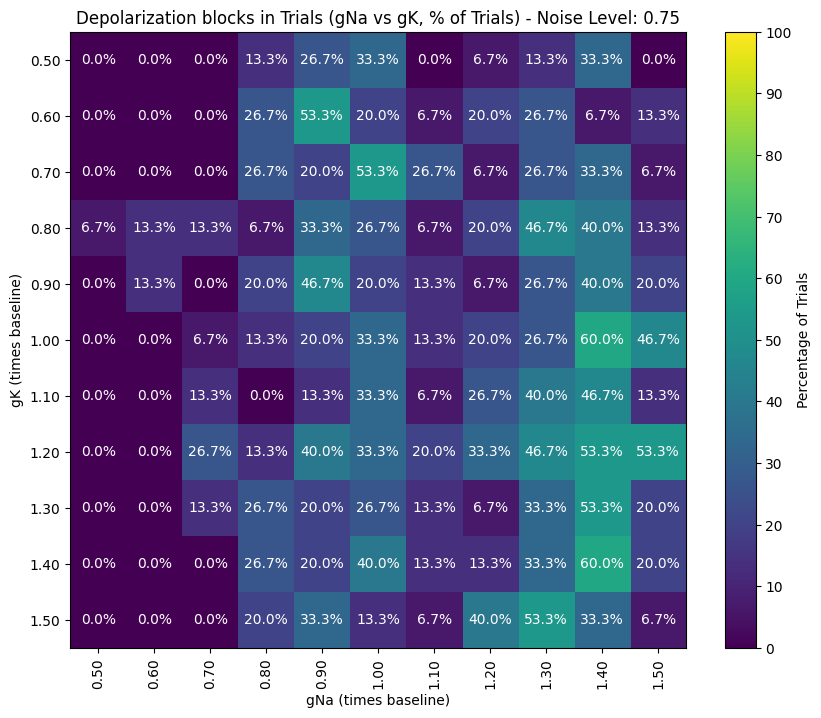
\includegraphics[width=\linewidth]{DPB_percentage_matrices/DPB_percentage_noise_0.75.png}
        \caption{} % Optional caption
    \end{subfigure}

    \bigskip % Adds vertical space between the rows

    % Row 2
    \begin{subfigure}{0.48\textwidth}
        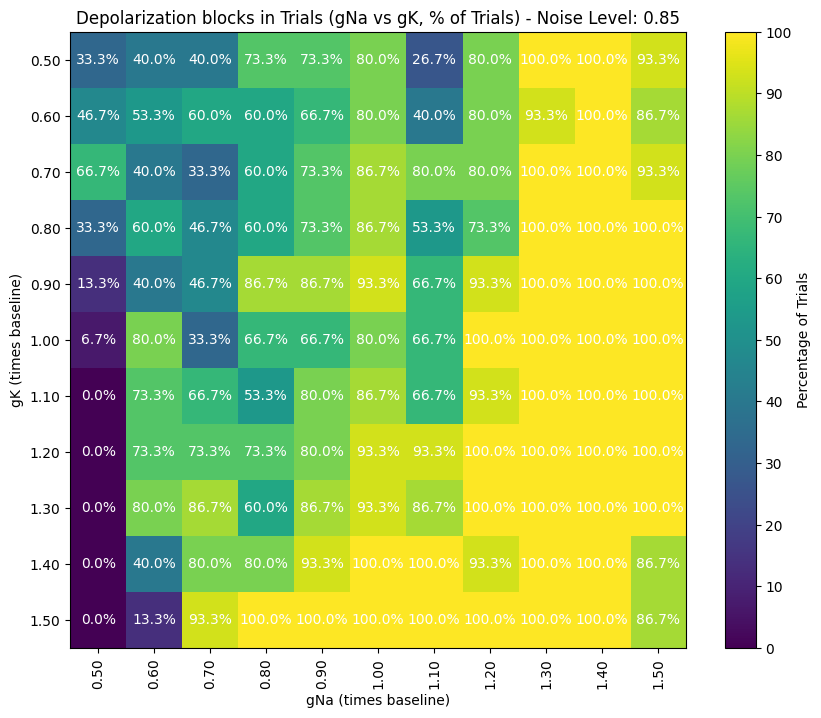
\includegraphics[width=\linewidth]{DPB_percentage_matrices/DPB_percentage_noise_0.85.png}
        \caption{} % Optional caption
    \end{subfigure}\hfill
    \begin{subfigure}{0.48\textwidth}
        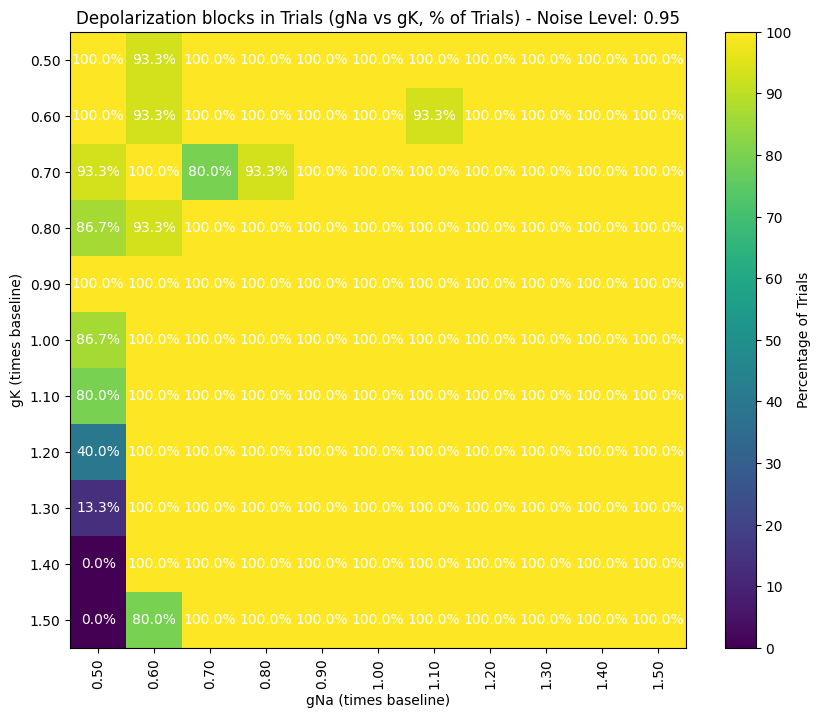
\includegraphics[width=\linewidth]{DPB_percentage_matrices/DPB_percentage_noise_0.95.png}
        \caption{} % Optional caption
    \end{subfigure}

    \caption[DPB percentage matrices]{Percentage of trials where depolarization block events occurred for all tested noise conditions.
        The x-axis shows all the sodium conductance changes in pyramidal cells, whereas the y-axis shows the potassium conductance changes in pyramidal cells.
        Modifications to pyramidal cells were applied to all compartments.
        The color intensity scales from 0 to 100 \%, where high-intensity yellow equals a higher amount of DPB events in a condition.
        The images are labeled from low noise to higher noise (a through d), respectively.}\label{fig:dpb_percentage_matrices}
\end{figure}

\subsection{Average delay of depolarization block events across noise conditions}
The average delay (+ standard deviation) of depolarization block (DPB) events was calculated in trials where these events occurred in Figure~\ref{fig:dpb_delay_matrices}.
These matrices showed similar trends to the DPB percentage matrices, with the average delay of DPB events being the shortest in the conditions where the most DPB events occurred.
These same conditions are associated with the the shortest average delay of DPB events and least standard deviation (\ref{fig:dpb_delay_matrices}, c and d).
The selected noise ranges are the same as in the percentage matrices, a percentage of the fixed 20x times baseline external noise level (0.65, 0.75, 0.85, 0.95).

\begin{figure}[htbp]
    \centering
    % Row 1
    \begin{subfigure}{0.48\textwidth}
        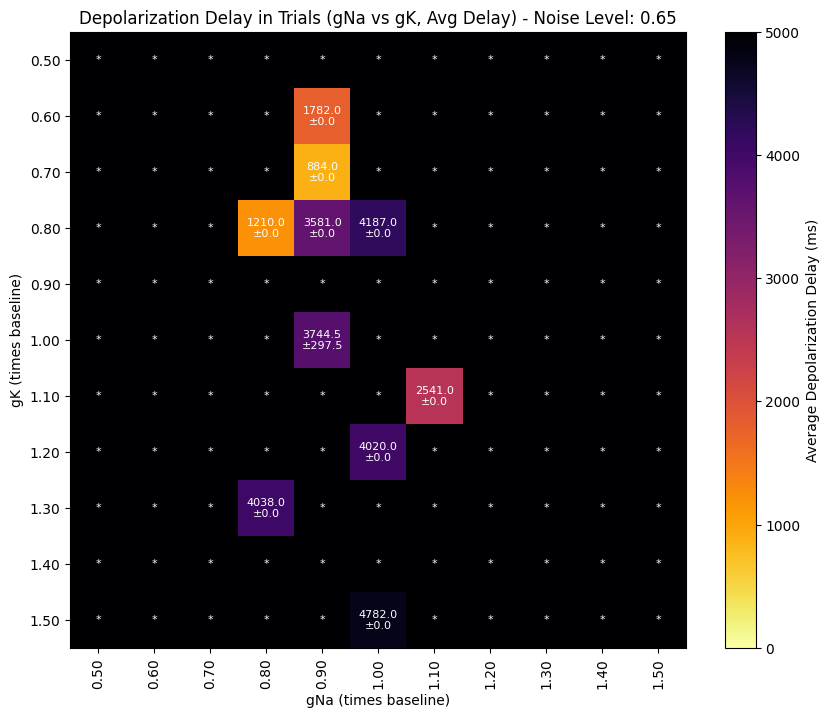
\includegraphics[width=\linewidth]{DPB_delay_matrices/DPB_delay_noise_0.65.png}
        \caption{} % Optional caption
    \end{subfigure}\hfill
    \begin{subfigure}{0.48\textwidth}
        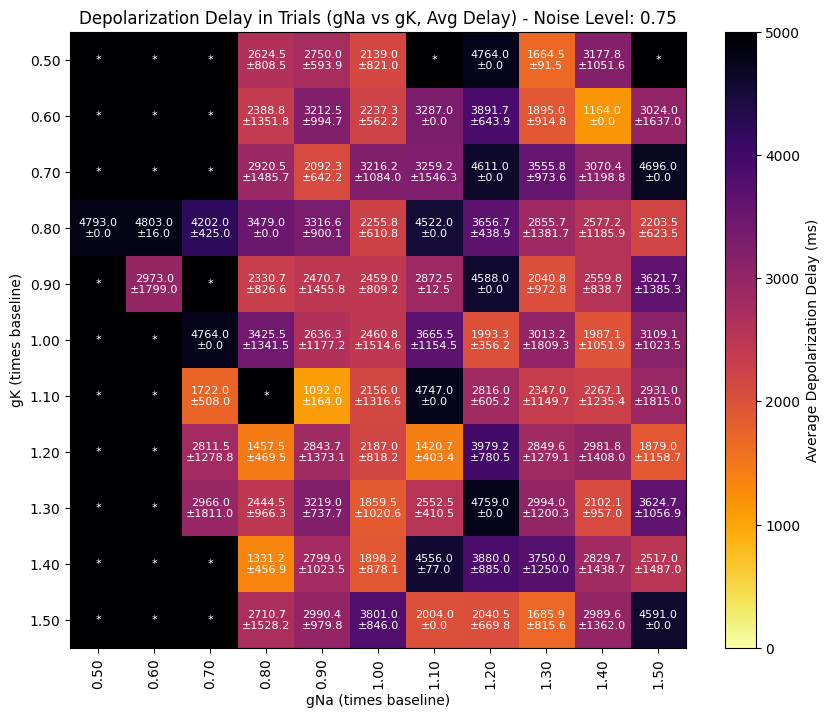
\includegraphics[width=\linewidth]{DPB_delay_matrices/DPB_delay_noise_0.75.png}
        \caption{} % Optional caption
    \end{subfigure}

    \bigskip % Adds vertical space between the rows

    % Row 2
    \begin{subfigure}{0.48\textwidth}
        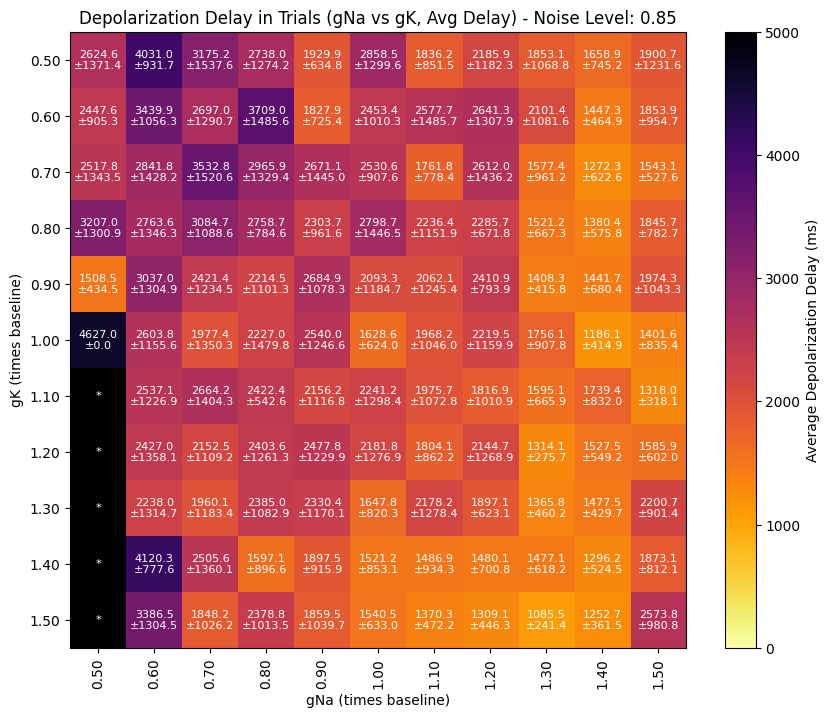
\includegraphics[width=\linewidth]{DPB_delay_matrices/DPB_delay_noise_0.85.png}
        \caption{} % Optional caption
    \end{subfigure}\hfill
    \begin{subfigure}{0.48\textwidth}
        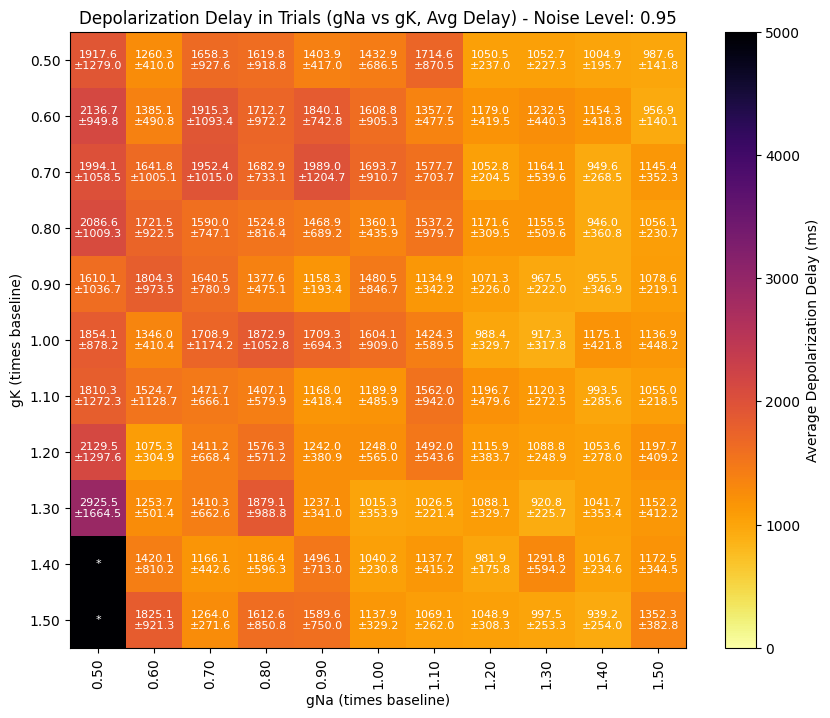
\includegraphics[width=\linewidth]{DPB_delay_matrices/DPB_delay_noise_0.95.png}
        \caption{} % Optional caption
    \end{subfigure}

    \caption[DPB delay matrices]{Average delay + Standard deviation of DPB in trials where depolarization block events occurred for all tested noise conditions.
        The x-axis shows all the sodium conductance changes in pyramidal cells, whereas the y-axis shows the potassium conductance changes in pyramidal cells.
        Modifications to pyramidal cells were applied to all compartments.
        The color intensity shows the average delay, where high-intensity red equals a shorter delay in DPB events in a condition.
        An asterisk (*) is an indication that no DPB events occurred in the condition and is colorless.
        The images are labeled from low noise to higher noise (a through d), respectively.}\label{fig:dpb_delay_matrices}
\end{figure}
\pagebreak

\section{Results of the External Noise: Burst analysis}
In addition to the depolarization block (DPB) analysis, the population bursts of pyramidal and basket neurons were analyzed near the onset of a DPB event.
Both peak height and general shape of the bursts were visualized in Figure~\ref{fig:burst_detection}.
The 2nd to last before, last burst before and 1st burst after the DPB event were detected and analyzed.
A range of sodium:potassium conductance changes in pyramidal cells were tested, namely: 1.00--1.00, 0.80--1.20, 1.20--0.80, and 1.20--1.20.
The external noise was fixed at 20x times the baseline of the original model.
Each burst has been aligned relative to the onset of the burst of the pyramidal population in the network (ms).
The bursts were averaged over 15 trials, and the standard deviation of the spike activity was visualized as a filled gradient surrounding the curve.

\subsection{Inter-ictal state}
For the baseline condition, in the inter-ictal state the 2nd to last burst before the depolarization block was detected.
The basket cell population burst occurred slightly before the pyramidal population burst with fairly low variance (\ref{fig:burst_detection}, a).
In all other conditions the basket cell burst occurred at least 50 ms after the pyramidal population burst.
The size of the basket cell burst only showed more variance in the 0.80--0.80 sodium:potassium condition (\ref{fig:burst_detection}, d), where the pyramidal burst also showed the most size variance.

\subsection{Pre-ictal state}
The pre-ictal network state shows the last burst before the depolarization block.
From the \textcite{sanjayImpairedDendriticInhibition2015} article, large external drive from the pyramidal population blocks basket cell firing.
Thus, the shift in basket cell burst timing is expected to be ahead of the pyramidal burst compared in the pre-ictal state.
In the baseline condition the pyramidal burst peaks right after the basket cell burst (\ref{fig:burst_detection}, a).
However, in all other conditions the basket cell burst shifts to further after the pyramidal burst, with the largest shift in the 1.20--1.20 sodium:potassium condition (\ref{fig:burst_detection}, e).
Again, the variance if the basket cell burst was very small compared to the pyramidal population (which is also four times larger than the basket cell population)

\subsection{Ictal state}
The ictal network state shows the first burst after the depolarization block, which only contained pyramidal activity in all conditions.
The shape of the pyramidal burst was fairly consistent across all conditions, in the 1.20--0.80 sodium:potassium condition the burst variance was slightly larger (\ref{fig:burst_detection}, c).
In addition this particular pyramidal burst lost its secondary peak, which was present in all other conditions.
All other conditions showed a secondary peak in the pyramidal burst, as the population spike activity became more desynchronized due to lack of somatic inhibition by the flat-lined basket cell activity (example of such population activity is visible in Figure~\ref{fig:example_burst_detection}).
The height of the pyramidal burst peak stayed consistent across all conditions.

\begin{figure}[htbp]
    \centering
    \includegraphics[width=0.95\textwidth]{burst_analysis_output.png}
    \caption[Burst detection near the onset of a depolarization block]{Analysis of burst detection
        before and after the onset of a depolarization block (DPB), showcasing the last two bursts before
        the DPB (Inter-ictal and Pre-ictal) and the first burst following it (Ictal). The figures (A-E)
        represent various sodium-potassium conductance ratios (\(g_{\text{Na}}\):\(g_{\text{K}}\)).
        A\@: 1.00--1.00, B\@: 0.80--1.20, C\@: 1.20--0.80, D\@: 1.20--1.20, E\@: 0.80--0.80.
        Bursts are aligned by the onset of pyramidal population activity, highlighted by the standard
        deviation in spike activity (shaded area). A dashed line in the Pre-ictal plot marks a
        comparative reference for timing shifts in the basket cell population.
        All plots share normalized y-axes to facilitate cross-comparison.
        Pyramidal neurons are depicted in blue and basket cells in green.}\label{fig:burst_detection}
\end{figure}
\pagebreak

\section{Results of the Recurrent Connections variants}
In this experiment, it was investigated if the network's susceptibility for depolarization block (DPB) events (ictal state) could be reduced by modifying the recurrent connection strength of basket cells.
The effects of stronger recurrent connections of basket cells was tested in conditions of sodium:potassium conductance combinations of pyramidal cells (+- 25 \% \(g_{\text{Na}}\) or \(g_{\text{K}}\)).
Steps of 5 \% increased recurrent connection strength were tested, ranging from 1.00 to 1.15 times the baseline connection strength (Figure~\ref{fig:rc_dpb_percentage_matrices}).

At baseline, all conditions showed the maximum amount of DPB events in the network (Figure~\ref{fig:rc_dpb_percentage_matrices}: a, 15 out of 15 trials or 100 \%).
Increasing the recurrent connection strength of basket cells by 5 \% led to slight decrease in the amount of DPB events in the network in 4 out of the 9 tested conditions (Figure~\ref{fig:rc_dpb_percentage_matrices}: b).
At 10 \% increased recurrent connection strength, the amount of DPB events decreased much strongly and some of the severe conditions only have DPB events in less than half of the trials (Figure~\ref{fig:rc_dpb_percentage_matrices}: c).
Lastly, at 15 \% increased recurrent connection strength, the amount of DPB events decreased even further, with some conditions showing no DPB events at all (Figure~\ref{fig:rc_dpb_percentage_matrices}: d).\\

\noindent More noise conditions are available for review in appendix~\ref{ch:appendix_c}.

\begin{figure}[htbp]
    \centering
    % Row 1
    \begin{subfigure}{0.48\textwidth}
        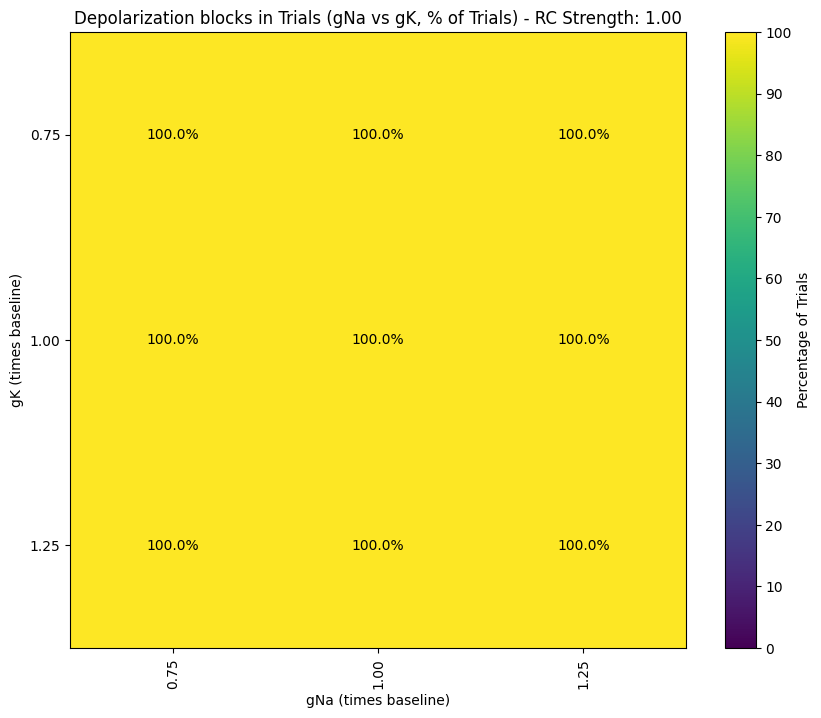
\includegraphics[width=\linewidth]{DPB_RC_Percentages/DPB_percentages_RC_1.00.png}
        \caption{} % Optional caption
    \end{subfigure}\hfill
    \begin{subfigure}{0.48\textwidth}
        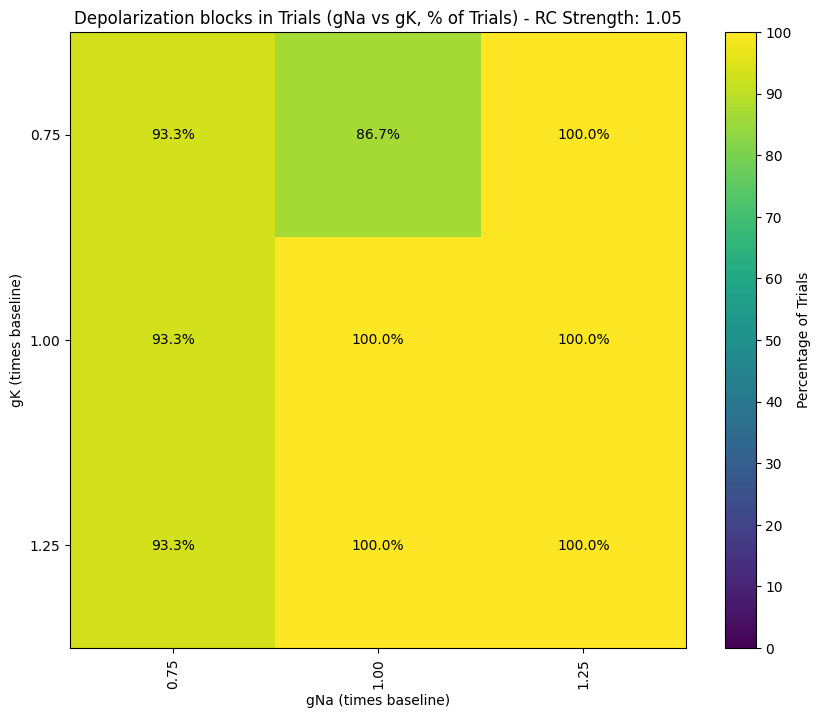
\includegraphics[width=\linewidth]{DPB_RC_Percentages/DPB_percentages_RC_1.05.png}
        \caption{} % Optional caption
    \end{subfigure}

    \bigskip % Adds vertical space between the rows

    % Row 2
    \begin{subfigure}{0.48\textwidth}
        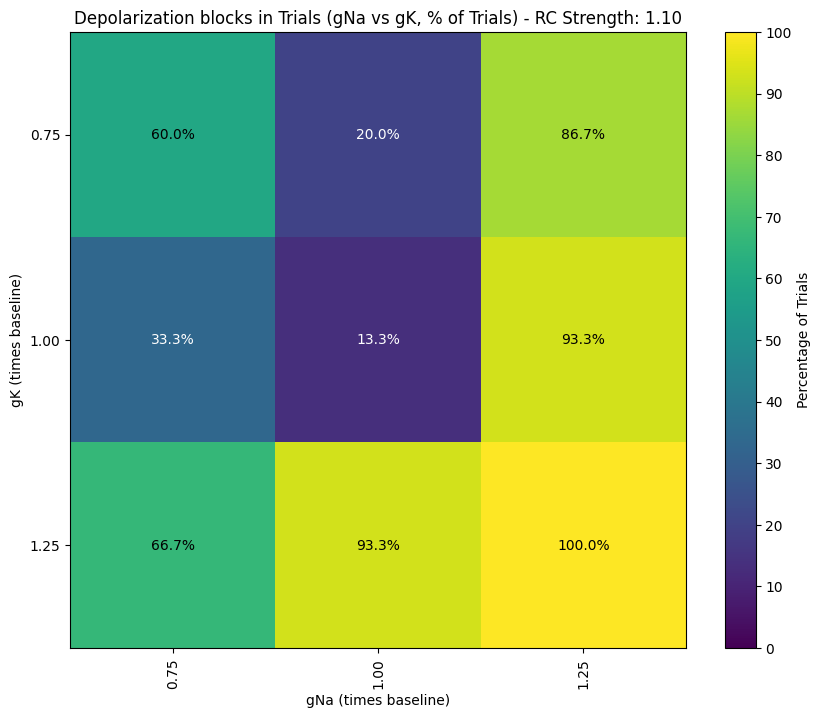
\includegraphics[width=\linewidth]{DPB_RC_Percentages/DPB_percentages_RC_1.10.png}
        \caption{} % Optional caption
    \end{subfigure}\hfill
    \begin{subfigure}{0.48\textwidth}
        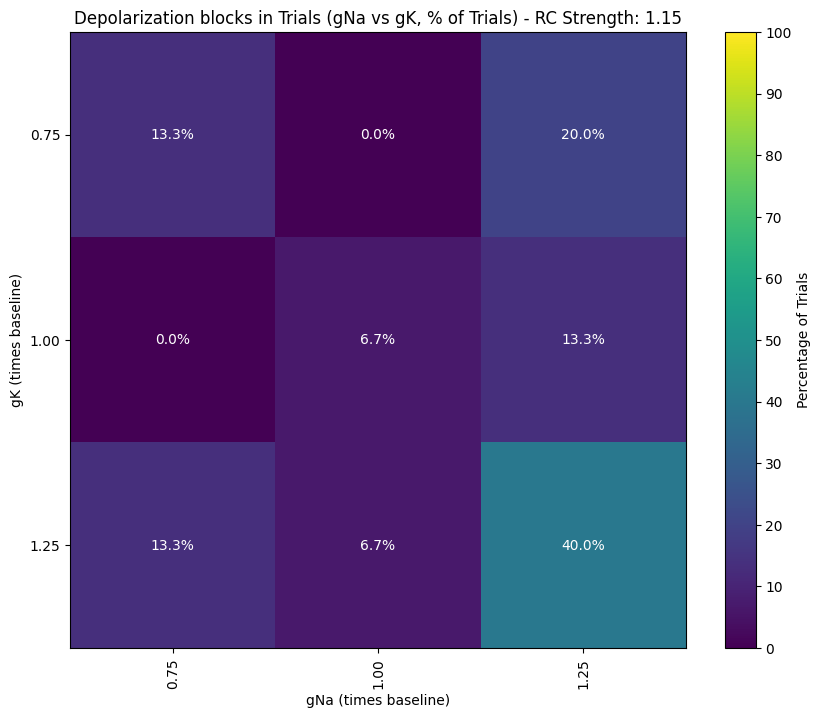
\includegraphics[width=\linewidth]{DPB_RC_Percentages/DPB_percentages_RC_1.15.png}
        \caption{} % Optional caption
    \end{subfigure}

    \caption[RC DPB percentage matrices (all)]{Percentage of trials where depolarization block events occurred for all tested noise conditions.
        The x-axis shows all the sodium conductance changes in pyramidal cells, whereas the y-axis shows the potassium conductance changes in pyramidal cells.
        Modifications to pyramidal cells were applied to all compartments.
        The color intensity shows the average delay, where high-intensity yellow equals higher percentage of DPB events in a condition.
        The images are labeled from low noise to higher noise (a through d), respectively.}\label{fig:rc_dpb_percentage_matrices}
\end{figure}